\documentclass{article} % For LaTeX2e
\usepackage{float}
\usepackage{nips,times}
\usepackage{url}
\usepackage[a4paper,bindingoffset=0.2in,%
            left=1in,right=1in,top=1in,bottom=1in,%
            footskip=.25in]{geometry} % let the margin be smaller.
\usepackage[hidelinks]{hyperref} % formate the url link
\usepackage{graphicx} % Required for the inclusion of images
\usepackage{natbib}
\setlength{\bibsep}{0.0pt}

\title{CS5340 Group13\\Hand Pose Estimation from Single Depth Images}

\author{
\begin{tabular}{ll}
Yang Xuan &  A0159066X\\
Liu Zhendong & A0159369L\\
Huang Mengying & A0159188M\\
\end{tabular}}

\newcommand{\fix}{\marginpar{FIX}}
\newcommand{\new}{\marginpar{NEW}}

\nipsfinalcopy

\begin{document}


\maketitle

\section{Overview}
This program implements Random Forest to do prediction for hand pose from single depth images, referencing the methods used in [1]. We have finished the ��Baseline-M�� that stated in [1]. Our dataset is downloaded from http://hpes.bii.a-star.edu.sg/index.php/instructions, which contains both training dataset and test dataset, 15 sub-directories respectively. Each of them contains information pertaining to various hand poses for different subjects. The goal of this report is to introduce what our team has done and propose what we plan to do in the future month. We will begin with the design of this program to show our understanding on the principles and our design to implement. We will continue by specifying the process of our implementation. Then, we will give a short conclustion to state what we have accomplished. Further, we will discuss about our future work.

So far we have our first version of the program including data pre-processing scripts, random forest and other essential codes, which was fully implemented by our group members using C++ with well written annotation and  documentation. Our source code can be viewed at github:
\newline
\\\url{ https://github.com/lzddzh/HandPoseEstimation}

\section{Design}
We design our program by three parts: preprocess, model training, prediction. Each one is following the paper [1], but with more detailed progress.
\subsection{Preprocess}
Our system adopts hand patch instead of individual pixel as one training examples. The original depth image in dataset contains background and other objects which are irrelevant to our hand pose estimation tasks, such as brackets of the data-glove device. Therefore, we need to obtain a hand-centered bounding box after preprocessing the image.
We first remove the background and noisy points by discarding the pixels of which depth value is greater than a certain threshold. Which means if a pixel��s depth is greater than the threshold, we directly set it��s value to be 32001 which is the maximum depth value.
Then we fixed the bounding box��s size to be $90\times 60$ and slide the windows through whole images to obtain the bounding box which contains the most ��non-background�� pixels. Here are some examples of image cropping.
\subsection{Model training}
We need to train a lot of decision trees for random forest and each tree has the same training process, so we only describe the procedure of training a decision tree.
\subsubsection{Depth features}
After preprocessing, each hand pose can be represented by following form: $E(X,Y)$ , where X is a $90\times 60$ dimension vector and Y is a $20\times 3$ dimension vector. Each dimension in X is calculated by�� . L is the 20 joint��s 3D position. So our goal is building a model based on the training examples and predicting the test example��s Y according to the corresponding X.
\subsubsection{Split criteria}
At each split node, we randomly choose a feature subset. For each feature, trying different split value to calculate information gain. Finally, we choose the best feature and split value which result in largest information gain to split this node into two children nodes. We only consider quantiles as our split value for the sake of efficiency. As for Entropy which is used to calculate information gain of a node, we use the entropy of multivariate Gaussian distribution like [1]. When calculating the Gaussian distribution, we add small random numbers to the diagonal of matrix  to make sure it is invertible, which means the determinant of the matrix can never equal to 0.
\subsection{Prediction}
Prediction of random forest is simply obtained by averaging the prediction from trees. So we only introduce how to obtain prediction from a decision tree here. Assume we represent an example as e(X,Y) .X is the feature vector and Y is the label vector. we let test example reach down to a certain leaf node L according to corresponding split features and split values which are selected during the model training phase. In current baseline model, we directly average all the training examples�� label vector in the leaf node L to generate prediction. But we have implemented the image similarity function which is based on the pixel gradient information. Later on, we can use this kind of similarity as vote weight for each training example in order to improve prediction accuracy.

\section{Implementation}
We implemented the whole random forest in C++ by ourselves. Two third party libraries are used. One is $Armadillo$ [2] to calculate the matrix covariance and determinant in information gain. Another is $OpenMP$ to enable our parallel training on multi-core computers. 

Below, we will introduce the structure of our code, the detailed methods we use to deal with specific difficulties.

\subsection{Data Pre-processing Scripts}
Like what we described in previous section, we will firstly convert the raw depth image into $90*60$ smaller image which contains only the hand and without many margin aside the hand. This work is done by Python using straight forward method. Then we want to gather all the images data into a single $.csv$ file instead of letting them each be separated on different files, since this will make our main program reading the training and test data easier.

In the .csv file, each line is the depth values of each pixels of a image divided by $','$, if the $.csv$ file is a training data set, then there will be 20 3D coordinates value following each line end, storing as 60 float numbers divided by $','$.

That is to say, each line of a .csv file is an example of training data or test data.

All these scripts are under the folder of $/scripts$.
\subsection{Main code}
Recall that in the previous section we stored the depth images into lines in a $.csv$ file. In each line, there are $90*60$ features and additional $20*3$ labels if the data is training data. Our main code task is to take such files as input, train the many tress in the random forest and using the trained tress to make predictions. 

We implemented our program in two modes, namely, debug and real time mode. In debug mode, we aim to adjust our code and parameters in the tree to get better prediction results. So we split the training data into two sub-datasets, $70\%$ for training and $30\%$ for predicting. Since the training data are all with labels, we can know the correct rate of our $30\%$ prediction. While in real time mode, we used the whole training data to train the random forest model and use the test data to get our prediction result. 

Written in C++, our code is naturally separated into below classes:

\begin{itemize}
\item Class $LoadData$:
\item Class $Node$: 
\item Class $Tree$: 
\item Class $RandomForest$:
\end{itemize}

Class $LoadData$ load training data or test from $.csv$ file into main memory and convert the raw depth value into features by the formula 7 in [1] section 3.2. This class also deal with the split operation of training data.

The Class $Node$ is the each node in the tree. Information stored in Node: 'Feature' that has been chosen at this node, 'Split point' that split the examples in this node into left branch and right branch. 'sub nodes' of this node, e.g. the left sub-node and the right sub-node. If the node is a leaf, then it will have 'label'.

Class $Tree$ contains the root node of the tree. We grow the tree and make prediction on a single tree at this class. This Class is using Class $Node$ as its tree nodes.

Class $RandomForest$: This class is the forest that perform a number of trees training and prediction, then the forest collect all the results and let the trees vote the final result. 

Besides the classes above, we have a main.cpp where we use the classes to load data, do training and make prediction.

Our core algorithm involving let the tree grow and choose the best split feature at a node is in the class $Tree$. In this class, a number of important functions are implemented:

\begin{itemize}
\item Function $learning(examples, feautres, depth)$:
\item Function $chooseBestFeature(features, examples)$:
\item Function $infoGain(examples, upSetExamples, downSetExamples)$
\item Function $printTree(Node, depth)$
\end{itemize} 

Function $Learning$ is implemented by a recursion way, each time the function will create a new node with its two sub-nodes and return the address of the new node to a previous call. Until the function $Learning$ find the examples numbers are to small(or meet other thresholds we set) then it will create a leaf node and no more grow this branch. 

Function $chooseBestFeature$ will try all the features to find a best one to split. For each feature, it will try $c$ times of split value to split the example set into two sets.
For now $c = 5$. 

Function $InfoGain$ calculates the information gain of the examples. In this function, matrix calculations are involved.

Function $printTree$ print the complete trained tree to console so we can see it when we are debugging. This function is implemented in a recursion way.

\subsection{Running Result}
A makefile is written in the folder of our program. After using "make" command, we will be able to run our program by "./run.out" in the terminal.

\begin{figure}[H]
\begin{center}
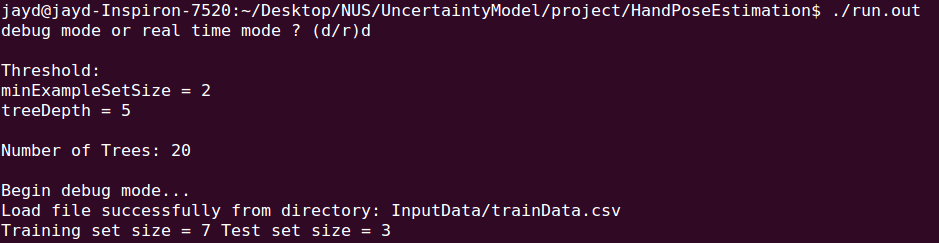
\includegraphics[width=0.6\textwidth]{output1} 
\caption{Console ouput of our program}
\end{center}
\end{figure}

Once you launch the program, it will ask you which mode to use, we choose 'debug' mode here. After the program finished, it will create result files containing the result of prediction under $/OutputData$ folder. And output the completed trees to the console.

\begin{figure}[H]
\begin{center}
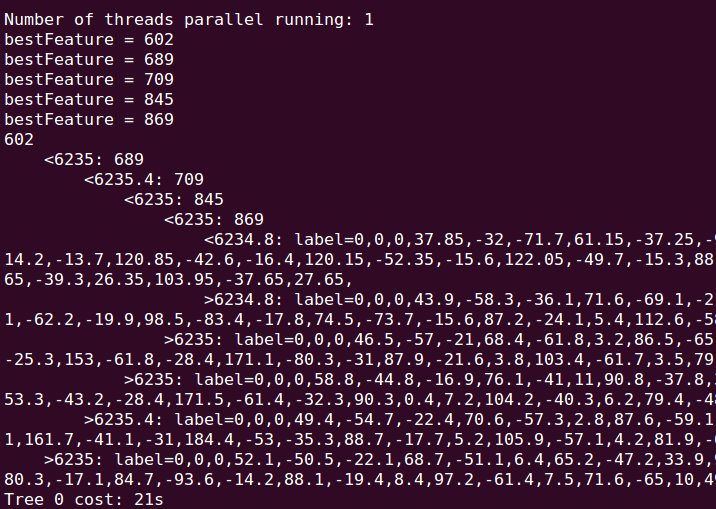
\includegraphics[width=0.6\textwidth]{output2} 
\caption{An example of printed tree}
\end{center}
\end{figure}

As Figure 2 shows, for now we are just using a depth of 5 tree and only 7 examples and cost 22 seconds to train such a tree. For more deep tree and whole training data training we will implement later.


\section{Conclusion}
Up to now we have trained each decision tree for the random forest successfully. But is on a small data set and the efficiency need to further improve. Besides, in the random forest, the vote is done by calculating the average value of all the results and uses average value of labels in each leaf node to do prediction, which is also referred to as Baseline-M in [1]. Now we can see that our design is basically feasible.

\section{Future Work}
Instead of making prediction with the empirical average as in Baseline-M, we will implement other methods to improve our prediction accuracy. As mentioned in [1], Baseline-S, during which static weights will be assigned to each training examples, but it remains unchanged during prediction stage. So, we would adopt a dynamically weighted scheme (i.e. DHand), where each of the weights can be decided at runtime. In depth image, the direction of the gradient indicates the higher depth value, so we can use gradient information to represent each pixel in an image. In the improved similarity computed function, sufficient statistics will be used to fully represent the raw input image hand image data, then execute bitwise OR operation to calculating the similarity score. Compared to empirical mean method, this dynamical weighted way can save huge storage memory because it does not need to store huge raw images. In the future month, we are going to improve our program from Baseline-M to DHand scheme. Meanwhile, we will make efforts to optimize our algorithms to speed the running time.

\section{References}

\bibliographystyle{unsrt}
\bibliography{refs}
\small{
[1] Chi Xu, Ashwin Nanjappa, Xiaowei Zhang, Li Cheng. {\it Estimate Hand Poses Efficiently from Single Depth Images}. In In International Journal of Computer Vision (IJCV), 2015.

[2] Conrad Sanderson and Ryan Curtin. {\it Armadillo: a template-based C++ library for linear algebra}. Journal of Open Source Software, Vol. 1, pp. 26, 2016.
}
\end{document}
